\documentclass[10pt]{article}
\usepackage[polish]{babel}
\usepackage[utf8]{inputenc}
\usepackage[T1]{fontenc}
\usepackage{amsmath}
\usepackage{amsfonts}
\usepackage{amssymb}
\usepackage[version=4]{mhchem}
\usepackage{stmaryrd}
\usepackage{graphicx}
\usepackage[export]{adjustbox}
\graphicspath{ {./images/} }

\title{GIMNAZJUM }

\author{}
\date{}


\newcommand\Varangle{\mathop{{<\!\!\!\!\!\text{\small)}}\:}\nolimits}

\begin{document}
\maketitle
\begin{enumerate}
  \item Odkurzacz-robot ma odkurzyć kwadratowy dywan o boku 20 m. Dywan podzielono na 400 kwadratów o boku 1 m , które odkurzacz czyści jeden po drugim, zgodnie z następującymi zasadami:
\end{enumerate}

\begin{itemize}
  \item jeśli pewien kwadrat został odkurzony, odkurzacz nie może ponownie wjechać na ten kwadrat
  \item odkurzacz jedzie cały czas w tym samym kierunku dopóki nie jest zmuszony, by zmienić kierunek, gdy natrafi na krawędź dywanu lub już odkurzony kwadrat
  \item gdy musi zmienić kierunek i ma do wyboru dwie opcje, może wybrać tę, którą chce.
\end{itemize}

Na początku odkurzacz jest umieszczony w jednym z kwadratów i może wybrać dowolny kierunek. Dla ilu kwadratów startowych będzie mógł wyczyścić cały dywan?\\
2. Wyznacz najmniejszą nieujemną liczbę całkowitą \(n\) taką, że \(n-2 \cdot Q(n)=2017\), gdzie \(Q(n)\) oznacza sumę cyfr liczby \(n\).\\
3. Dzień nazwiemy szczęśliwym, jeżeli jego zapis w formacie DD.MM.RRRR zawiera osiem parami różnych cyfr, gdzie DD oznacza dzień, MM miesiąc, a RRRR - rok oraz dla dni i miesięcy o numerach mniejszych od 10 za pierwszą cyfrę przyjmujemy zero. Przykładowo 26.04.1785 był dniem szczęśliwym. Kiedy nadejdzie najbliższy (licząc od dzisiaj) szczęśliwy dzień?

\section*{LICEUM}
\begin{enumerate}
  \item Punkty A, B, C, D, E, F leżą w tej kolejności, zgodnie z ruchem wskazówek zegara, na okręgu w taki sposób, że \(A D\) jest średnicą tego okręgu. Prosta BF przecina proste AD i CD odpowiednio w punktach G i H, przy czym \(\Varangle F E H=54^{\circ}, \Varangle D E C=31^{\circ}\), oraz \(\Varangle D G B=128^{\circ}\).Znajdź \(\Varangle C E B\).
  \item Osiem osób - cztery kobiety i ich mężowie - wzięło udział w N imprezach. Wiemy, że żadna para małżonków nie wzięła udziału w tej samej imprezie, a każda para nie-małżonków (włączając pary tej samej płci) wzięła razem udział w dokładnie jednej imprezie. Ponadto jedna z osób była tylko na dwóch imprezach. Jaka jest najmniejsza wartość N, dla której taka sytuacja jest możliwa?
  \item Trójkąt \(A B C\), w którym \(A B=A C=5 m\) oraz \(B C=6 m\), jest częściowo wypełniony wodą. Gdy trójkąt leży na boku \(B C\), poziom powierzchni wody znajduje się 3 m ponad bokiem. Na jakiej wysokości w metrach znajduje się powierzchnia wody, gdy trójkąt leży na boku AB?\\
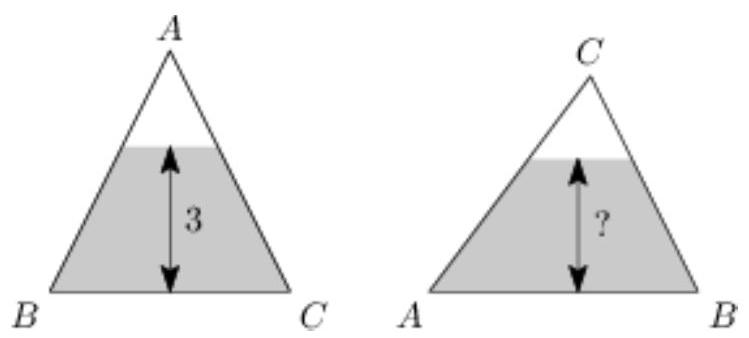
\includegraphics[max width=\textwidth, center]{2024_11_21_bd352e229c34ad64190bg-1}
\end{enumerate}

\end{document}